\documentclass{beamer}

\usepackage[utf8]{inputenc} % Language and font encoding
\usepackage[icelandic]{babel}
\usepackage[T1]{fontenc}


\usepackage{tikz}
\usepackage[listings,theorems]{tcolorbox}
\usepackage{booktabs}
\usepackage{minted} %Minted and configuration
\usemintedstyle{default}

\renewcommand{\theFancyVerbLine}{\sffamily \arabic{FancyVerbLine}}
%%%%%%%%%%%
% More math
%%%%%%%%%%%
\newcommand{\Mod}[1]{\ \text{mod}\ #1}

%%%%%%%%%%%%%%%%%%%%%%
% Beamer configuration
%%%%%%%%%%%%%%%%%%%%%%
\setbeamertemplate{navigation symbols}{}
\usecolortheme{dove}
\setbeamercolor{frametitle}{fg=white}

\usebackgroundtemplate%
{%
\vbox to \paperheight{

\includegraphics[width=\paperwidth]{Pics/hi-slide-head-2016}

\vfill
\hspace{0.5cm}
\includegraphics[width=0.3\paperwidth]{Pics/hi-von-logo}
\vspace{0.4cm}
    }%
}

\AtBeginSection[]
{
  \begin{frame}<beamer>
    \frametitle{Yfirlit}
    \tableofcontents[currentsection]
  \end{frame}
}

\setbeamerfont{frametitle}{size=\normalsize}
\addtobeamertemplate{frametitle}{}{\vspace*{0.5cm}}

%%%%%%%%%%%%%%%%%%%%%%%%%
% tcolorbox configuration
%%%%%%%%%%%%%%%%%%%%%%%%%

% Setup from: http://tex.stackexchange.com/a/43329/21638
\tcbset{%
    noparskip,
    colback=gray!10, %background color of the box
    colframe=gray!40, %color of frame and title background
    coltext=black, %color of body text
    coltitle=black, %color of title text 
    fonttitle=\bfseries,
    alerted/.style={coltitle=red, colframe=gray!40},
    example/.style={coltitle=black, colframe=green!20, colback=green!5},
}


%%%%%%%%%%%%%%%%%%%%%%%
% Further configuration
%%%%%%%%%%%%%%%%%%%%%%%
\hypersetup{colorlinks=true,pdfauthor={Eirikur Ernir Thorsteinsson},linkcolor=blue,urlcolor=blue}
\graphicspath{{./Pics/}}

\author{Eiríkur Ernir Þorsteinsson}
\institute{Háskóli Íslands}
\date{Haust 2016}

\title{Stærðfræðimynstur í tölvunarfræði}
\subtitle{Vika 7, fyrri fyrirlestur}

\begin{document}

\begin{frame}
\titlepage
\end{frame}


\section{Inngangur}

\begin{frame}{Í síðasta tíma}
\begin{itemize}
 \item Endurkvæm reiknirit
 \begin{itemize}
  \item Endurkvæmni og ítrun
  \item Merge sort reikniritið
 \end{itemize}
 \item Rökstudd forritun
\end{itemize}
\end{frame}

\section{Talning}

\begin{frame}{Talning}
\begin{columns}
\column{0.5\textwidth}
\begin{itemize}
 \item Talning á ýmsum hlutum kemur víða við
 \begin{itemize}
  \item Höfum þegar framkvæmt talningu, t.d. á fjölda grunnaðgerða í reikniritum
 \end{itemize}
 \item Getum sett fram reglur um talningu á ýmsum fyrirbrigðum
\end{itemize}
\column{0.5\textwidth}
\begin{center}
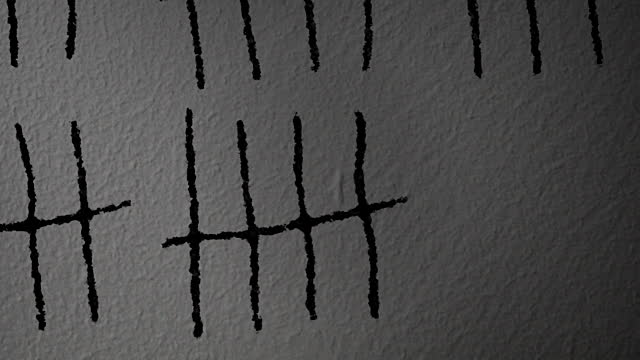
\includegraphics[width=\linewidth]{counting}
\end{center}
\end{columns}
\end{frame}

\begin{frame}{Um framsetningu}
\begin{itemize}
 \item Fjórar reglur verða settar fram
 \item Í hverri þeirra er talað um uppskiptingu á ``vandamálum'' eða ``verkefnum''
 \item Hér er það þó fjöldinn sem skiptir máli, ekki akkúrat eðli ``verkefnisins''
\end{itemize}
\end{frame}


\begin{frame}{Margfeldisreglan}
\begin{tcolorbox}[title=Margfeldisreglan]
Brjótum verkefni niður í tvö undirverkefni. Séu $n_1$ mismunandi leiðir til að gera fyrra undirverkefnið og séu, fyrir hvert fyrra undirverkefnið, $n_2$ leiðir til að gera seinna undirverkefnið, þá eru $n_1 \cdot n_2$ leiðir til að gera allt verkefnið.
\end{tcolorbox}
\end{frame}

\begin{frame}{Dæmi}
Fyrirtæki með starfsfólkið Sanchez og Patel, leigja skrifstofuhúsnæði með 12 skrifstofum. Á hve marga vegu geta Sanchez og Patel fengið aðskildar skrifstofur?
\pause

\vspace{1cm}
Við getum skipt verkinu í skref - fyrst látum við Sanchez velja skrifstofu, svo látum við Patel velja skrifstofu. Sanches hefur úr 12 möguleikum að velja, Patel 11. Fjöldi möguleika sem þau geta skipt skrifstofunum á milli sín er þá $11 \cdot 12 = 132$.
\end{frame}

\begin{frame}{Dæmi}
Hversu margir mismunandi bitastrengir af lengd 7 eru til?
\pause

\vspace{1cm}
Hver bitanna sjö getur verið valinn á tvo mismunandi vegu (0 eða 1). Margfeldisreglan segir þá að til séu $2^7 = 128$ mismunandi bitastrengir af lengd 7.
\end{frame}

\begin{frame}{Dæmi}
\begin{itemize}
 \item Hversu margar mismunandi númeraplötur er hægt að framleiða ef númerin samanstanda af\ldots
 \begin{itemize}
  \item Tveimur enskum bókstöfum (26 möguleikar) og svo þremur tölustöfum (10 möguleikar)? \pause
  \begin{itemize}
   \item $26^2 \cdot 10^3 = 676000$
  \end{itemize}
  \item Þremur enskum bókstöfum og svo tveimur tölustöfum? \pause
  \begin{itemize}
   \item $26^3 \cdot 10^2 = 1757600$
  \end{itemize}
  \item Tveimur enskum bókstöfum og svo fjórum tölustöfum? \pause
  \begin{itemize}
   \item $26^2 \cdot 10^4 = 6760000$
  \end{itemize}
 \end{itemize}
 \item Hvað segir þetta okkur um val á lykilorðum? \pause
 \begin{itemize}
  \item Hafið þau löng!
 \end{itemize}
\end{itemize}
\end{frame}

\begin{frame}{Summureglan}
\begin{tcolorbox}[title=Summureglan]
Skoðum verkefni sem er þess eðlis að valið sé á milli tveggja undirverkefna þannig að aðeins þurfi að vinna annað verkefnið. Séu $n_1$ mismunandi leiðir til að gera annað undirverkefnið og $n_2$ leiðir til að gera hitt undirverkefnið, þá eru $n_1 + n_2$ leiðir til að gera allt verkefnið.
\end{tcolorbox}
\end{frame}

\begin{frame}{Dæmi}
Velja þarf fulltrúa í háskólaráð, sem annað hvort má vera kennari eða nemandi. Ef það eru 37 kennarar og 1234 nemendur, hve marga valkosti höfum við ef við gerum ráð fyrir enginn sé bæði nemandi og kennari?
\pause
\[
 37+1234 = 1271
\]
\end{frame}

\begin{frame}{Summureglan og mengi}
Við getum tengt summuregluna við mengi. Séu $A$ og $B$ sundurlæg þá gildir $|A \cup B| = |A| + |B|$. Einnig,
\[
 |A_1 \cup A_2 \cup \ldots \cup A_n| = |A_1| + |A_2| + \ldots + |A_n|
\]
að því tilskildu að fyrir öll $i,j$ gildi $i \neq j \to A_i \cap A_j = \emptyset$. Þetta gildir ekki hafi mengin sameiginleg stök.
\end{frame}

\begin{frame}{Frádráttarreglan}
\begin{tcolorbox}[title=Frádráttarreglan]
Megi vinna verkefni með annaðhvort einni af $n_1$ aðferðum eða með einni af $n_2$ aðferðum, þá er heildarfjöldi leiða til að vinna verkið $n_1 + n_2$ að frádregnum þeim fjölda leiða sem eru sameiginlegar í upptalningunum.
\end{tcolorbox}
Sem kemur ekki á óvart því að
\[
 |A \cup B| = |A| + |B| - |A \cap B|
\]

\end{frame}

\begin{frame}{Deilingarreglan}
\begin{tcolorbox}[title=Deilingarreglan]
Séu $n$ aðferðir til að vinna verk en fyrir hverja niðurstöðu séu nákvæmlega $d$ aðferðir sem leiða til hennar þá er fjöldi niðurstaðna $\frac{n}{d}$.
\end{tcolorbox}
\end{frame}

\begin{frame}{Dæmi}
Hvað eru margar aðferðir til að raða fjórum manneskjum í fjóra stóla? \pause Notum margfeldisreglu:
\[4! = 24\]
En ef við röðum stólunum við hringborð og gerum ekki greinarmun á uppröðunum þar sem sama manneskja hefur sama sætisfélaga til vinstri og hægri? \pause Notum deilingarreglu:
\[\frac{4!}{4} = 6\]
\end{frame}


\section{Skúffureglan}

\begin{frame}{Skúffureglan}
\begin{tcolorbox}[title=Skúffuregla Dirichlets]
Látum $k$ vera jákvæða heiltölu. Séu $k + 1$ hlutir settir í $k$ skúffur, þá inniheldur a.m.k. ein skúffan meira en einn hlut.
\end{tcolorbox}

Dæmi: Ef við setjum 20 sokka í 19 skúffur, þá mun a.m.k. ein skúffan innihalda tvo eða fleiri sokka.
\end{frame}

\begin{frame}{Skúffureglan}
Skúffureglan er venjulega kölluð ``The Pigeonhole Principle'' á ensku, og útskýrð með $k+1$ dúfum sem fljúga í $k$ holur.
\begin{center}
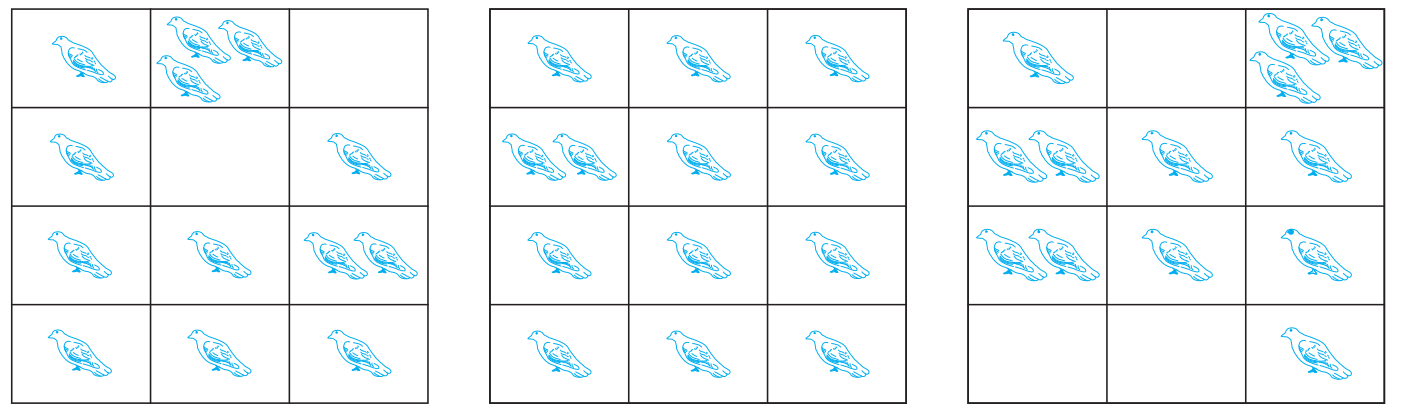
\includegraphics[width=\textwidth]{pigeons}
\end{center}
\end{frame}

\begin{frame}{Skúffureglan - afleiðingar}
Skúffuregluna má nota til að rökstyðja ýmsar fullyrðingar sem upp koma í talningafræði, t.d.
\begin{tcolorbox}
Fall $f$ með $k+1$ staka formengi og $k$ staka bakmengi er ekki eintækt.
\end{tcolorbox}
\end{frame}

\begin{frame}{Dæmi}
\begin{itemize}
 \item Í stofu með 367 nemendur eiga tveir nemendur sama afmælisdag
 \item Í 27 orða enskri setningu byrja tvö orðanna á sama bókstaf
 \item Séu einkunnir gefnar á heiltöluskalanum 0 til 10 fá tveir nemendur sömu einkunn sé fjöldi nemenda 12 eða hærri
\end{itemize}
\end{frame}

\begin{frame}{Almenna skúffureglan}
Við getum sett fram almennari skúffureglu (e. \emph{generalized pigeonhole principle}) til að segja til um hversu margir hlutir eru í hverri skúffu:
\begin{tcolorbox}[title=Almenna skúffureglan]
Séu $N$ hlutir settir í $k$ kassa, þá inniheldur a.m.k. einn kassi $\left\lceil \frac{N}{k}\right\rceil$ hluti.
\end{tcolorbox}
Dæmi: Í hópi 100 fólks eru a.m.k. $\left\lceil \frac{100}{12}\right\rceil = 9$ sem eiga afmæli í sama mánuði.

\end{frame}

\begin{frame}{Næst}
6.3 (Umraðanir), 6.4 (Tvíliður).

Ef tími gefst verður byrjað á 8. kafla. (Ekki sjöunda!)
\end{frame}


\end{document}
